TODO: 3.5, 3.6, 3.7, 3.8, 3.9, 3.10, 3.11, 3.12

%%% AUTHOR : BERTRAND GOBBERS %%%

\section*{3.1: A linear circuit}

\begin{figure}[htbp]
\begin{center}
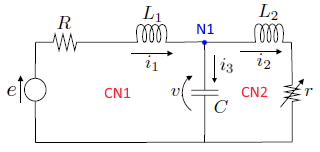
\includegraphics[height=4cm]{ex31}
\end{center}
\end{figure}

As we have seen in section 3.4, the state variables of an electrical network usually are the currents in the inductances and the voltages across the capacitors. We can thus define 3 state variables :

\begin{equation}
\begin{split}
&x_1 = i_1\\
&x_2=i_2\\
&x_3=v
\end{split} 
\end{equation}

The two inputs are defined as the input voltage $e$ and the variable resistor $r$ so we have :

\begin{equation}
\begin{split}
&u_1 = e\\
&u_2=r
\end{split} 
\end{equation}


In this circuit, by grouping the dipoles in series, we have $N=2$ nodes and $M=3$ branches.\\

We have thus $N-1=1$ current equations by applying Kirchhoff's current law on node N1, with $i_3$ defined as the current flowing through capacitor C :

\begin{equation}
i_1 =i_2+i_3 =i_2 + C \frac{dv}{dt} = i_2 + C\dot{v}
\end{equation}




We also have $M-N+1=2$ voltage equations by applying Kirchhoff's voltage law on closed networks CN1 and CN2 :

\begin{equation}
\begin{split}
&e - Ri_1 - L_1 \frac{di_1}{dt}-v=e - Ri_1 - L_1 \dot{i_1}-v=0\\
&v-L_2 \frac{di_2}{dt} - ri_2 = v-L_2 \dot{i_2} - ri_2=0
\end{split} 
\end{equation}

From these state equations, we can find the following state model :


\begin{equation}
\begin{split}
&\dot{x_1} = \frac{1}{L_1} (u_1 - Rx_1-x_3)\\
&\dot{x_2} = \frac{1}{L_2} (x_3-u_2x_2)\\
&\dot{x_3} = \frac{1}{C} (x_1-x_2)
\end{split}
\end{equation}

\newpage

\section*{3.2: A voltage doubler bridge}

\begin{figure}[htbp]
\begin{center}
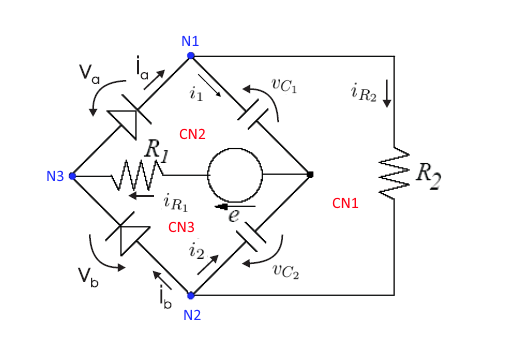
\includegraphics[scale=0.8]{ex32}
\end{center}
\end{figure}

As usual, we can define the 2 state variables as the voltages across the 2 capacitors :

\begin{equation}
\begin{split}
&x_1 = v_{C_1}\\
&x_2=v_{C_2}
\end{split} 
\end{equation}

We define the voltage-current characteristics of the 2 diodes as $i_a=f(v_a)$ for the upper diode and $i_b=f(v_b)$ for the lower diode.\\

In this circuit, we have $N=4$ nodes and $M=6$ branches.\\

We have thus $N-1=3$ current equations by applying Kirchhoff's current law on nodes N1, N2 and N3 :

\begin{align}
\label{t1}
&i_1+i_{R_2}-i_a = 0 \quad \Rightarrow \quad C_1\dot{v_{C_1}} = -i_{R_2}+f(v_a)\\
\label{t2}
&i_2+i_b-i_{R_2} = 0 \quad \Rightarrow\quad C_2\dot{v_{C_2}} = i_{R_2}-f(v_b)\\
\label{t4}
-&i_a+i_{R_1}+i_b = 0 \quad \Rightarrow \quad i_{R_1} = f(v_a)-f(v_b)
\end{align}


We also have $M-N+1=3$ voltage equations by applying Kirchhoff's voltage law on closed networks CN1, CN2 and CN3 :

\begin{align}
\label{test}
v_{C_2}+v_{R_2}-v_{C_1} & = 0\\
\label{t6}
e - v_{R_1} - v_a - v_{C_1} & = 0\\
\label{t5}
e - v_{R_1} + v_b - v_{C_2} & = 0
\end{align}

From (\ref{test}) and knowing that $v_{R_2}=R_2 i_{R_2}$ we can find the following expression : 
\begin{equation}
\label{t3}
i_{R_2}=\frac{v_{C_1}-v_{C_2}}{R_2}
\end{equation}

By replacing (\ref{t3}) in (\ref{t1}) and (\ref{t2}), we can find :

\begin{align}
&C_1\dot{v_{C_1}} = \frac{v_{C_2}-v_{C_1}}{R_2}+f(v_a)\\
&C_2\dot{v_{C_2}} = \frac{v_{C_1}-v_{C_2}}{R_2}-f(v_b)
\end{align}

We can see that the state model is established if we can express the variables $v_a$ and $v_b$ as a function of the state variables $v_{C_1}$ and $v_{C_2}$. Knowing that $v_{R_1}=R_1i_{R_1}$ and using (\ref{t4}), we can find the following new expressions for (\ref{t6}) and (\ref{t5}) :

\begin{align}
-e + R_1\left(f(v_a)-f(v_b)\right) + v_a + v_{C_1} & = 0\\
-e + R_1\left(f(v_a)-f(v_b)\right) - v_b + v_{C_2} & = 0
\end{align}

We can express the Jacobian matrix of these expressions, as a function of the variables $v_a$ and $v_b$ :

\begin{equation}
J=
\begin{pmatrix}
\frac{\partial F_1(v_a,v_b)}{\partial v_a} & \frac{\partial F_1(v_a,v_b)}{\partial v_b} \\
\frac{\partial F_2(v_a,v_b)}{\partial v_a} & \frac{\partial F_2(v_a,v_b)}{\partial v_b} \\
\end{pmatrix}\\
=\begin{pmatrix}
R_1 \frac{df(v_a)}{dv_a}+1 & -R_1 \frac{df(v_b)}{dv_b} \\
R_1 \frac{df(v_a)}{dv_a} & -R_1 \frac{df(v_b)}{dv_b}-1 \\
\end{pmatrix}\\
\end{equation}

We can see that $det(J) \neq 0$ because $\frac{df(v_a)}{dv_a} \geq 0$ and $\frac{df(v_b)}{dv_b} \geq 0$ $\forall v_a, v_b$. By applying the implicit function theorem, there are two functions $g_a$ and $g_b$ such that $v_a=g_a(v_{C_1},v_{C_2},e)$ and $v_b=g_b(v_{C_1},v_{C_2},e)$. Hence the following state model :

\begin{align}
&C_1\dot{v_{C_1}} = \frac{v_{C_2}-v_{C_1}}{R_2}+f(g_a(v_{C_1},v_{C_2},e))\\
&C_2\dot{v_{C_2}} = \frac{v_{C_1}-v_{C_2}}{R_2}-f(g_b(v_{C_1},v_{C_2},e))
\end{align}

Which gives, by replacing the state variables :

\begin{align}
&\dot{x_1} = \frac{1}{C_1} \left( \frac{x_2-x_1}{R_2}+f(g_a(x_1,x_2,e)) \right)\\
&\dot{x_2} = \frac{1}{C_2} \left( \frac{x_1-x_2}{R_2}-f(g_b(x_1,x_2,e)) \right)
\end{align}

\newpage

\section*{3.3: A transformer}

\begin{figure}[htbp]
\begin{center}
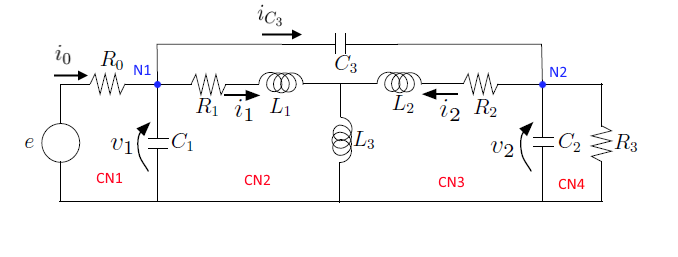
\includegraphics[scale=0.8]{ex33}
\end{center}
\end{figure}

\noindent \textbf{1.}
In this circuit, we have a capacitor \blue{mesh}\footnote{A mesh is a closed network without repetition of nodes.} formed by $C_1$, $C_2$ and $C_3$. Therefore, we can define 2 state variables as the voltages across $C_1$ and $C_2$, $v_1$ and $v_2$. Here, we don't need the voltage across $C_3$ as a state variable because it is redundant with $v_1$ and $v_2$. Indeed, $v_{C_3} = v_1-v_2$.\\

In this circuit, we also have a \blue{cut}\footnote{A cut is an ensemble of branches whose extraction will split an associated network in at least two associated separate sub-networks.} of inductance formed by $L_1$, $L_2$ and $L_3$. Therefore, we can define 2 state variables as the currents flowing through $L_1$ and $L_2$, $i_1$ and $i_2$. Here, we don't need the current flowing through $L_3$ as a state variable because it is redundant with $i_1$ and $i_2$. Indeed, $i_{L_3}=i_1+i_2$.\\

We thus have 4 state variables : $i_1$, $i_2$, $v_1$, $v_2$.\\

\noindent \textbf{2.}
First, we can develop the expression of the currents flowing through the capacitors and resistors and the voltages across the inductances :

\begin{equation}
\begin{split}
&i_{C_1}= C_1 \dot{v_1}\\
&i_{C_2}= C_2 \dot{v_2}\\
&i_{C_3}= C_3 \left( \dot{v_1} - \dot{v_2}\right)\\
&i_{R_3} = \frac{v_2}{R_3}\\
&v_{L_1}= L_1 \dot{i_1}\\
&v_{L_2}= L_2 \dot{i_2}\\
&v_{L_3}= L_3 \left( \dot{i_1} + \dot{i_2} \right)
\end{split} 
\end{equation}

In this case, if we proceed as before (writing N-1 current equations and M-N+1 voltage equations), we will have many redundant equations. We will thus have to select useful equations to get our state model.\\

\newpage

We can begin by using Kirchhoff's current law on nodes N1 and N2 :

\begin{align}
\label{t9}
i_0 - C_1 \dot{v_1} + C_3 \left( \dot{v_1} - \dot{v_2}\right) + i_1 & = 0\\
\label{t10}
i_2 + C_2 \dot{v_2} + \frac{v_2}{R_3} - C_3 \left( \dot{v_1} - \dot{v_2}\right) & = 0
\end{align}

Then, we can use Kirchhoff's voltage law on closed networks CN1, CN2, CN3 and CN4 :

\begin{align}
\label{t11}
e-R_0i_0-v_1 & = 0\\
\label{t12}
v_1-R_1i_1- L_1 \dot{i_1} - L_3 \left( \dot{i_1} + \dot{i_2} \right) & = 0\\
\label{t13}
v_2-R_2i_2- L_2 \dot{i_2} - L_3 \left( \dot{i_1} + \dot{i_2} \right) & = 0\\
\label{t14}
v_2-R_3i_{R_3} & = 0
\end{align}

From (\ref{t12}) and (\ref{t13}), we can write the first part of the state model :


\begin{equation}
\begin{pmatrix}
L_1+L_3 & -L_3\\
L_3 & -(L_2+L_3)
\end{pmatrix}
\begin{pmatrix}
\dot{i_1}\\
\dot{i_2}
\end{pmatrix}
=
\begin{pmatrix}
-R_1 & 0 & 1 & 0\\
0 & -R_2 & 0 & 1
\end{pmatrix}
\begin{pmatrix}
i_1\\
i_2\\
v_1\\
v_2
\end{pmatrix}\\
\end{equation}

By isolating $i_0$ in (\ref{t9}), $i_{R_3}$ in (\ref{t10}) and replacing their value in (\ref{t11}) and (\ref{t14}), we can find the second part of the state model :

\begin{equation}
\begin{pmatrix}
R_0(C_1+C_3) & -R_0C_3\\
-R_3C_3 & R_3(C_2+C_3)
\end{pmatrix}
\begin{pmatrix}
\dot{v_1}\\
\dot{v_2}
\end{pmatrix}
=
\begin{pmatrix}
-R_0 & 0 & -1 & 0\\
0 & -R_3 & 0 & -1
\end{pmatrix}
\begin{pmatrix}
i_1\\
i_2\\
v_1\\
v_2
\end{pmatrix}\\
+
\begin{pmatrix}
1\\
0
\end{pmatrix}
e
\end{equation}

\newpage

\section*{3.4: A circuit with a tunnel diode}

The circuit for which we have to draw the schematic is described by the 2 following state equations :

\begin{equation}
\begin{split}
&C\dot{x_1} = -h(x_1)+x_2\\
&L\dot{x_2} = -x_1 - Rx_2 + u
\end{split} 
\end{equation}

The first equation is a current equation while the second is a voltage equation (therefore, the input u is a voltage). By looking at these equations, we know that our circuit will be constituted of 5 elements :\\

\begin{itemize}
\item[•] A voltage source
\item[•] A resistor R
\item[•] A capacitor C
\item[•] An inductance L
\item[•] A tunnel diode\\
\end{itemize}

We know from the first equation that the current flowing through L will divide at a node in two currents : one flowing through C and one flowing through the tunnel diode. We also know that the voltage across C is also the voltage across the tunnel diode.\\

From the second equation, we know that the resistor R is in series with the inductance L. We also know that the input voltage u, the resistor R, the inductance L and the capacitor C form together a closed network. Therefore, we can draw the following schematic for our circuit :

\begin{figure}[htbp]
\begin{center}
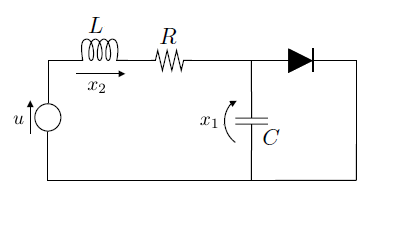
\includegraphics[scale=0.8]{ex34}
\end{center}
\end{figure}